% Traducción revisada sobre el original inglés y el borrador de Anahi.

% DOCX paragraph 192
\chapter{El espaciotiempo, la curvatura y la gravedad}\label{ch:03}
\chaptermark{Espaciotiempo, curvatura y gravedad}

% DOCX paragraph 193
% Title continued in paragraph 192.

% DOCX paragraph 196
Este capítulo tiene la audaz ambición de explicar de manera sencilla una serie de conceptos
abstractos que subyacen a la teoría de la relatividad general de Einstein. Las matemáticas de
esta teoría pueden expresar esos conceptos de forma transparente y elegante, y un físico o un
matemático lo ve (casi) todo claro una vez se han anotado las ecuaciones correspondientes. O
sea que yo podría simplemente enseñárselas y decir: «está todo ahí, ¿no lo veis?» Sé, sin
embargo, que este enfoque no nos llevaría muy lejos, habiéndome comprometido con el lector, o
la lectora, a actuar como un guía vigilante a lo largo de este viaje.\index{relatividad general}

% DOCX paragraph 197
Bien, lo que voy a hacer es, desde luego, más difícil: ilustrar esta nueva interpretación de la
gravedad empleando conceptos a los que todos estamos habituados. El desafío de este
planteamiento está relacionado no tanto con la complejidad de los conceptos (todo eso está en
las matemáticas) como con el esfuerzo necesario para aceptar una interpretación de la realidad
física que a menudo contrasta con nuestra experiencia cotidiana. En otras palabras, lo que pido
es que los lectores se imaginen una realidad que puede estar muy alejada de aquello a lo que
están acostumbrados. Pero por otra parte, la imaginación es uno de los requisitos de este
viaje.

% DOCX paragraph 198
Comencemos pues allí donde terminó el capítulo anterior, a saber, cuando dijimos que las
ecuaciones de Einstein resumen con elegancia la equivalencia entre la gravedad y la curvatura
del espaciotiempo. Para ser más precisos, escribimos que estas ecuaciones esencialmente afirman
que:\index{curvatura}

% DOCX paragraph 200
\begin{equation}\label{eq:03-01}
\begin{pmatrix}\text{la gravedad es la manifestación} \\ \text{de la curvatura del espaciotiempo}\end{pmatrix}
\end{equation}

% DOCX paragraph 201
% Equation number is generated with the preceding equation.

% DOCX paragraph 203
Sé por experiencia —y de leer las caras de demasiados estudiantes cuando la escribo por primera
vez en la pizarra— que esta frase suena fundamentalmente oscura. Y sin embargo, es correcta y
absolutamente verídica, al menos en la medida en que podemos verificarlo mediante experimentos
científicos. Que no desesperen los lectores y, sobre todo, que no se rindan ahora. Más
adelante, cuando volvamos a esta afirmación, se verán capaces de comprenderla e incluso de
apreciar sus profundas implicaciones.

% DOCX paragraph 206
\section[El espaciotiempo]{El espaciotiempo: todo lo que ha ocurrido y ocurrirá}\label{sec:03-spacetime}

% DOCX paragraph 208
Para comprender lo que realmente dice la ecuación \eqref{eq:03-01}, podemos analizar los
diversos términos que contiene. Empecemos con el concepto de espaciotiempo. En primer lugar,
nótese que no he escrito «espacio-y-tiempo» ni «espacio-tiempo», sino «espaciotiempo». Tal vez
parezca una diferencia mínima, irrelevante, pero no lo es; es fundamental porque representa una
de las primeras lecciones de la teoría de la relatividad general. Se debe a que Einstein
postula que nuestra idea del espacio y el tiempo en cuanto entidades distintas es incorrecta,
ya que ambos son completamente equivalentes. Se sigue de ahí que un desplazamiento en el
espacio de un punto a otro es equivalente a nivel de las ecuaciones, a un desplazamiento en el
tiempo de un momento a otro. Ir a la izquierda o a la derecha, arriba o abajo, no es en
absoluto distinto, al menos matemáticamente, de ir atrás o adelante en el tiempo.

% DOCX paragraph 209
En la teoría de Einstein, por tanto, el espaciotiempo es un único objeto que puede verse en
esencia como un «contenedor» de elementos (es decir, lo que en matemáticas se llama «conjunto»)
a los que también nos referimos como sucesos. Lo explico con un ejemplo: la Unión Europea puede
considerarse un conjunto de ciudadanos de diversos países; estos ciudadanos son pues los
ladrillos, o elementos, de la Unión Europea. Análogamente, el espaciotiempo es el conjunto de
todos los sucesos: pasados, presentes y futuros. Un suceso (un elemento del espaciotiempo) se
entiende como algo que ha ocurrido, está ocurriendo o ocurrirá en algún sitio en algún momento.
El despertador que pusiste esta mañana, el desayuno, tomar un autobús al trabajo… Todo eso son
sucesos. Estar leyendo este libro en este momento también es un suceso, ya que es posible
establecer que ocurre en un determinado sitio (por ejemplo en tu sofá) en un momento específico
(ahora). Como cada suceso necesita que se especifiquen cuatro tipos de información (tres para
la posición en el espacio y uno para el tiempo) es fácil concluir que el espaciotiempo es un
contenedor de cuatro dimensiones (tres espaciales y una temporal) de elementos, llamados
sucesos.\index{suceso (espaciotiempo)}

% DOCX paragraph 210
A esta definición, Einstein añade que este contenedor de sucesos no es muy útil si se toma por
sí solo sin más reglas. Por tanto es necesario establecer unas reglas precisas para identificar
la posición relativa de los diversos elementos, es decir su distancia. En otras palabras,
cuando consideramos dos sucesos A y B, es esencial que establezcamos en qué relación están
entre ellos, o sea, si A ocurrió antes o después de B, si está a su derecha o a su izquierda,
encima o debajo y por último, si los dos están conectados de alguna manera o por el contrario
son completamente independientes.

% DOCX paragraph 211
Estas reglas solo pueden establecerse eligiendo las coordenadas, es decir, después de
introducir una serie ordenada de números que establecen la secuencia de sucesos y de esa manera
nos permiten conocer la posición relativa de A y B. Esta elección de coordenadas es totalmente
arbitraria, de ahí el adjetivo relatividad en la teoría de Einstein, pero las relaciones entre
los sucesos que se desprenden de la elección de coordenadas son las mismas, independientemente
de la elección que se haya hecho. Esta es la razón por la cual, dentro de la teoría de la
relatividad general, sigue siendo posible establecer sin ambigüedad lo primero que hiciste esta
mañana: despertarte o desayunar.\textsuperscript{\hyperlink{note:03-01}{1}} Además, la
secuencia de sucesos será la misma para todos los observadores, cualquiera que sea su estado de
movimiento.\index{coordenadas}

% DOCX paragraph 214
\section{Curvatura}\label{sec:03-curvature}

% DOCX paragraph 216
Ahora que entendemos lo que es el espaciotiempo, regresemos a nuestra ecuación \eqref{eq:03-01}
y centrémonos en el segundo concepto que figura ahí, el de la curvatura.\index{curvatura}

% DOCX paragraph 217
Una vez más, las matemáticas nos ofrecen herramientas sofisticadas y elegantes para medir la
curvatura de una superficie en un espacio de dimensiones arbitrarias. Sin entrar en detalles,
lo que necesitamos saber aquí es que hay superficies que pueden considerarse «curvadas» y que
su grado de curvatura puede medirse usando herramientas matemáticas bastante simples, una de
las cuales es el concepto de transporte paralelo en un circuito cerrado. Así es como funciona:
tómese un vector (una «flecha» de determinada longitud) en una determinada porción del
espaciotiempo y muévase a lo largo de un bucle cerrado, asegurándose de que siempre apunte en
la misma dirección. Si hacemos esto, realizamos un transporte paralelo, y hay un objeto
matemático (llamado tensor de Riemann o de curvatura) que medirá la cantidad de curvatura
presente al ir alrededor del bucle.\index{transporte paralelo}\index{vector}\index{curvatura!transporte paralelo}\index{curvatura!tensor (Riemann)}\index{tensor!Riemann}\index{tensor!curvatura}

% DOCX paragraph 218
Esto tal vez suene abstracto, pero unos ejemplos ayudarán a verlo más claro. Consideremos pues
una superficie en dos dimensiones, empezando con la más sencilla posible, un plano. A
continuación, imaginemos que el circuito cerrado está representado mediante un triángulo ABC y
que usamos, como referencia para una determinada dirección una flecha de longitud dada cuyo
origen coincide con el punto A y cuya dirección está alineada con el lado AB. En matemáticas y
física, una flecha de este tipo se llama «vector» y se caracteriza por una longitud y una
dirección indicadas por la punta de la flecha. Ahora podemos deslizar nuestro vector a lo largo
de AB, llevarlo al punto B y desplazarlo hacia el punto C. Al hacer esto, es importante
mantener fija la dirección inicial de la flecha, dado que en eso consiste el transporte
paralelo. Una vez en C, transportaremos el vector al lado AC y cerraremos el circuito, como se
muestra en la figura~\ref{fig:03-01}.\index{vector}

% DOCX paragraph 221
\begin{figure}[htbp]
\centering
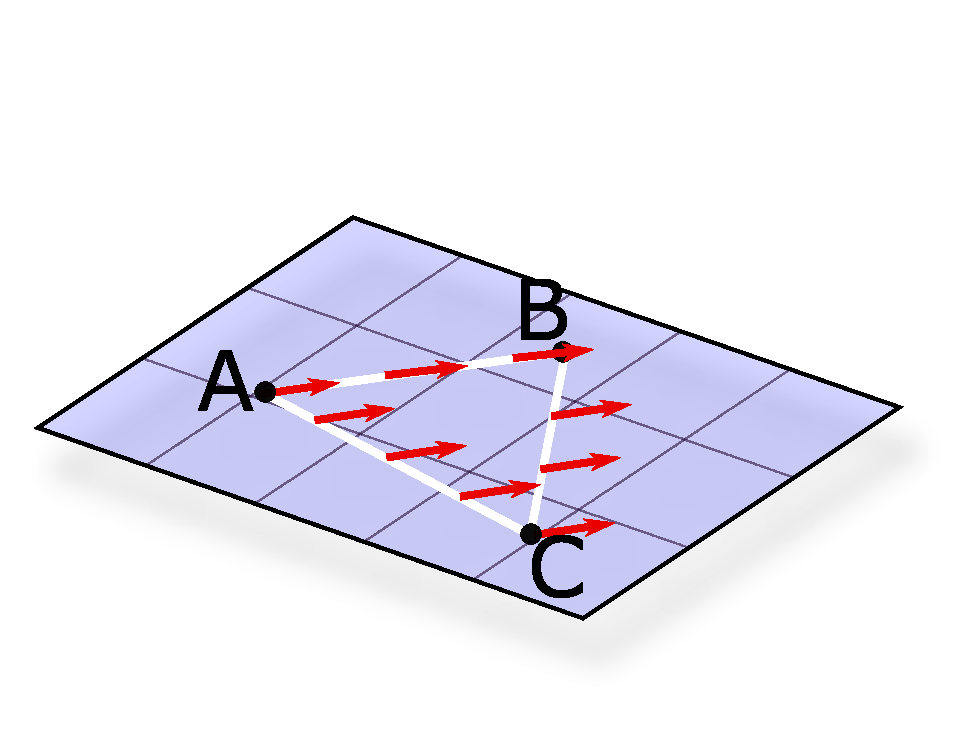
\includegraphics[width=0.88\linewidth,height=0.48\textheight,keepaspectratio]{../figs/pdf/en/fig-03-01.pdf}

% DOCX paragraph 222
\caption{\emph{Transporte paralelo de una flecha (vector) a lo largo del triángulo ABC en un plano
bidimensional. La comparación entre el vector final y el inicial en A nos muestra que son
idénticos: el plano es una superficie plana porque tiene curvatura cero.}}\label{fig:03-01}
\end{figure}



% DOCX paragraph 223
Llegados a este punto, podemos comparar el vector final con el inicial, y concluimos que son
idénticos: nada ha cambiado por llevarlo paralelo a lo largo de un circuito cerrado contenido
en un plano. Además, diremos que esta ausencia de cambio en los dos vectores está relacionada
con la ausencia de curvatura en la superficie, es decir que el plano es una superficie plana
porque tiene curvatura cero.\index{vector}\index{espaciotiempo!plano}\index{curvatura!nula (plano)}

% DOCX paragraph 224
Lo siguiente que necesitamos es un ejemplo de una superficie no plana. Consideremos una
superficie bidimensional que los matemáticos adoran por su sencillez y por la riqueza de
propiedades: una esfera bidimensional, es decir, la superficie de una esfera con radio
constante. Podemos pensar en una esfera bidimensional como la cáscara de una naranja, pero que
fuera lisa y muy fina, o bien en una representación simplificada de la superficie de la Tierra.\index{esfera bidimensional}

% DOCX paragraph 225
En este caso, podríamos construir un circuito cerrado (de nuevo representado por el triángulo
ABC) conectando dos meridianos (líneas de longitud) a través de la sección de un paralelo
(línea de latitud) que los intersecta. Imaginemos pues que salimos del punto A, quizás una
hermosa isla en el Caribe, y apuntamos al norte con ayuda de una brújula. Mientras nos movamos
siguiendo la aguja con exactitud, esencialmente estamos llevando nuestro vector paralelo a lo
largo del meridiano y por tanto podemos alcanzar el Polo Norte, es decir el punto B. Allí,
teniendo cuidado de no dar la vuelta, mirando siempre en la misma dirección, nos vamos en
dirección sur siguiendo otro meridiano, por ejemplo el que está situado formando un ángulo
recto con el primero, y así llegamos al punto C en algún sitio del norte de África. Una vez
llegados a nuestro destino, a la latitud de A, nos trasladamos dirección oeste a lo largo del
paralelo que forma el lado CA del triángulo pero siempre mirando en la dirección en la que
alcanzamos el Polo Norte.\index{vector}

% DOCX paragraph 226
Llegados de nuevo a A y habiendo cerrado el circuito, tal como se aprecia en la
figura~\ref{fig:03-02}, podemos comparar el vector final con el inicial y concluimos que esta
vez no son idénticos en absoluto: apuntan en direcciones perpendiculares, el primero al norte y
el segundo al este.\index{vector}

% DOCX paragraph 228
\begin{figure}[htbp]
\centering
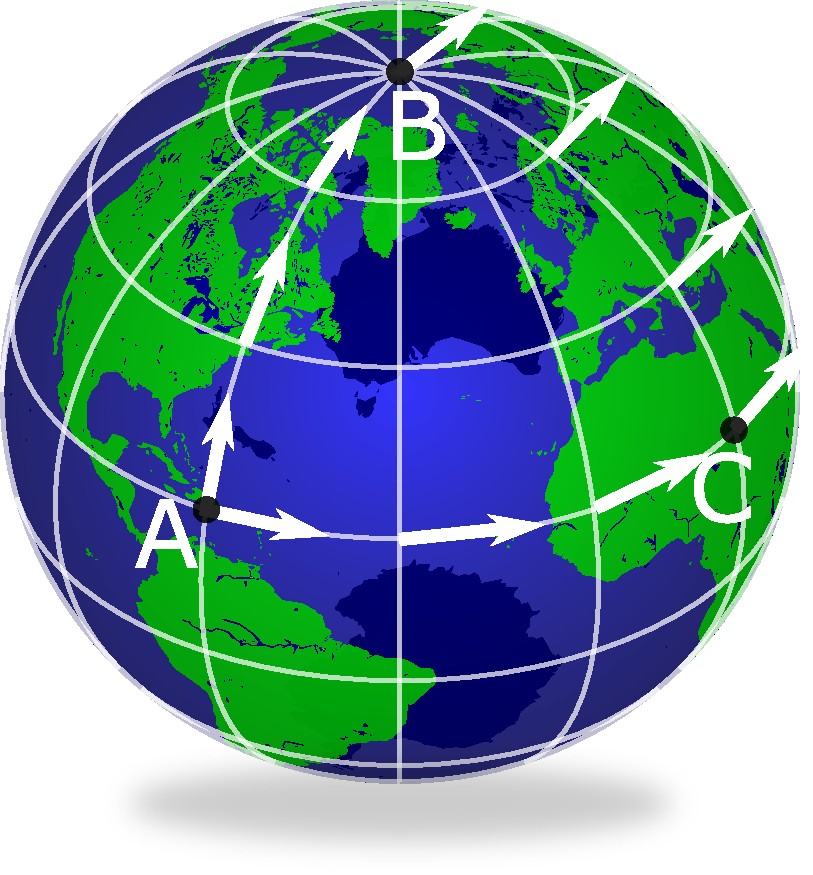
\includegraphics[width=0.88\linewidth,height=0.48\textheight,keepaspectratio]{../figs/pdf/en/fig-03-02.pdf}

% DOCX paragraph 229
\caption{\emph{Transporte paralelo de un vector a lo largo de un circuito cerrado en una esfera bidimensional.
La comparación entre el vector final y el inicial muestra que los dos son diferentes porque
apuntan en direcciones perpendiculares: la esfera bidimensional es una superficie curvada y
tiene curvatura no nula.\index{esfera bidimensional}}}\label{fig:03-02}
\end{figure}



% DOCX paragraph 230
De esta manera, hemos visto que el transporte paralelo de un vector a lo largo de un bucle
cerrado en una esfera bidimensional introduce un cambio en la dirección de un vector y que este
cambio está relacionado con la presencia de una curvatura en la superficie esférica. En otras
palabras, hemos aprendido que una esfera bidimensional es una superficie curvada porque tiene
curvatura no nula.\index{transporte paralelo}\index{esfera bidimensional}\index{vector}\index{espaciotiempo!curvado}\index{curvatura!no nula (curvado)}

% DOCX paragraph 231
Por supuesto que este simple experimento debería ser suficiente para convencer a los
terraplanistas de lo insensata que es su teoría. Pero también revela algo muy interesante y nos
invita a una serie de importantes reflexiones. La primera es que si hubiéramos elegido un
triángulo muy pequeño, la variación entre los dos vectores habría sido menos evidente. Por
ejemplo, si hubiéramos considerado un triángulo con lados de tan solo cien metros, habría sido
muy difícil medir la diferencia entre los vectores sin unas herramientas muy sofisticadas. Por
tanto, una superficie curva se puede aproximar, al menos localmente (es decir, en la vecindad
de cada uno de sus puntos), por una superficie plana. Dicho con otras palabras, los efectos de
la curvatura solo son evidentes en escalas comparables a lo que se llama radio de curvatura de
la superficie curvada.\index{espaciotiempo!plano (localmente)}\index{espaciotiempo!radio de curvatura}

% DOCX paragraph 232
Para entender mejor este punto y simplificarlo en gran medida, podemos decir que siempre es
posible aproximar, al menos localmente, una superficie curvada con una esférica. En este caso,
la esfera bidimensional que aproxima la superficie curvada (también llamada superficie
osculante) tendrá un radio igual al radio local de la curvatura de la superficie curvada. Así,
si nos limitamos a una superficie en una sola dimensión espacial (es decir, una curva de
dimensión uno), una curva así siempre se puede aproximar localmente con una circunferencia cuyo
radio representa el radio local de la curvatura.\index{esfera bidimensional}\index{superficie!osculante}\index{curvatura!radio}

% DOCX paragraph 233
Esto se ilustra en la figura~\ref{fig:03-03}, donde la línea negra muestra un corte
unidimensional de una superficie bidimensional curvada genérica. Claramente, si nos movemos de
izquierda a derecha, la curvatura a lo largo de la línea varía de un punto a otro; podemos
suponer, sin embargo, que en cada punto, o región alrededor de un punto, podemos encontrar un
círculo (una esfera bidimensional en la superficie bidimensional) que aproxima, al menos
localmente, la línea. Debería estar igual de claro que los radios de esos círculos son todos
diferentes y que allí donde la línea es localmente recta, el radio del círculo puede llegar a
ser muy grande y no se muestra en la figura.\index{esfera bidimensional}

% DOCX paragraph 235
\begin{figure}[htbp]
\centering
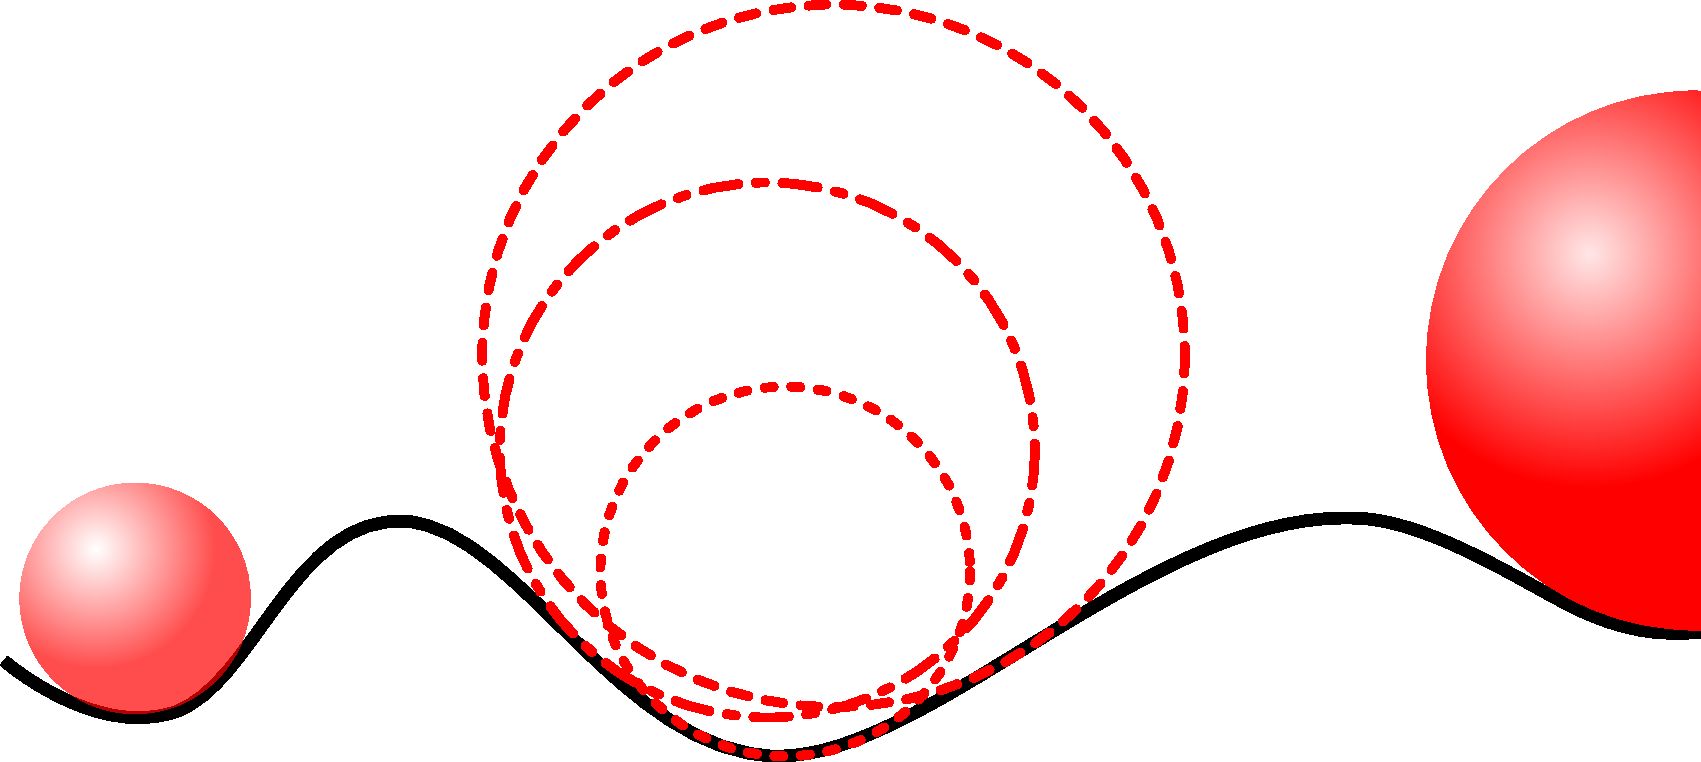
\includegraphics[width=0.88\linewidth,height=0.48\textheight,keepaspectratio]{../figs/pdf/en/fig-03-03.pdf}

% DOCX paragraph 237
\caption{\emph{La línea negra representa un corte de dimensión uno de una superficie bidimensional curvada genérica. La
curvatura a lo largo de la línea varía de un punto a otro pero siempre se puede aproximar
localmente por un círculo (una esfera bidimensional en la superficie bidimensional). Los radios
de los círculos pueden variar y ser muy grandes si la línea es casi recta.\index{curvatura!radio}\index{esfera bidimensional}}}\label{fig:03-03}
\end{figure}



% DOCX paragraph 239
Si, por otra parte, quisiéramos considerar el espaciotiempo en sus cuatro dimensiones,
tendríamos que emplear una esfera de cuatro dimensiones (y yo soy el primero en admitir que es
difícil de imaginar) osculando en cada punto la curvatura local del espaciotiempo de dimensión
cuatro.\index{esfera!osculante}

% DOCX paragraph 240
Dadas estas consideraciones, no resultará sorprendente que una superficie plana (que como hemos
visto es una superficie con curvatura cero) tenga también un radio de curvatura asociado a
ella, aunque este radio es infinito. En el caso de la Tierra, el radio de curvatura es igual a
su radio, es decir, unos 6400 kilómetros, razón por la cual es necesario considerar escalas tan
grandes como la distancia del Caribe al Polo Norte para medir la diferencia entre los vectores.
Si hubiéramos realizado el experimento en una plaza tan grande como la plaza de San Marcos en
Venecia, medir una diferencia entre los dos vectores habría sido muchísimo más difícil, aunque
no imposible con la tecnología actual.\index{curvatura!radio (Tierra)}\index{vector}

% DOCX paragraph 241
La segunda consideración, desencadenada por el transporte paralelo en una esfera bidimensional,
se desprende directamente de la primera y nos enseña una noción fundamental que usaremos con
gran frecuencia durante este viaje. Debido a que nuestra experiencia del mundo físico se
desarrolla en escalas de longitud de unas pocas decenas de kilómetros (nuestra vista no llega
mucho más lejos) y está construida basada en el campo gravitatorio presente en la Tierra,
resulta casi inevitable desarrollar la percepción de que las leyes de la física son las de un
espaciotiempo plano, es decir, con curvatura cero. Pero eso es una impresión incorrecta, igual
que lo es suponer que la superficie de la Tierra es plana solo porque es difícil apreciar su
curvatura. Afortunadamente, la intuición de Einstein fue lo suficientemente profunda para
deshacerse de las restricciones de nuestra percepción del espaciotiempo plano. Volveremos a
este punto en el siguiente capítulo.\index{transporte paralelo}\index{esfera bidimensional}\index{percepcion@percepción}

% DOCX paragraph 242
La tercera consideración es que la herramienta matemática que hemos empleado hasta ahora (el
transporte paralelo de un vector a lo largo de un circuito cerrado) es completamente general y
por tanto se puede aplicar también a superficies cuya curvatura es mucho más compleja que las
que hemos visto hasta ahora. Si nos fijamos en la figura~\ref{fig:03-04}, vemos una superficie
bidimensional cuya curvatura es diferente en cada punto, excepto en las regiones alejadas del
centro. En particular, si se piensa en el radio local de curvatura, es muy pequeño cerca del
origen y aumenta de tamaño a medida que te alejas del centro. Exactamente en el origen, el
radio de curvatura es infinito porque la función que he elegido al representar la superficie
bidimensional (es decir, sin(r)/r) tiene un valor constante de aproximadamente uno cerca del
origen. Por último, el ejemplo de la figura~\ref{fig:03-04} muestra que la curvatura puede
incluso cambiar de signo, hacerse positiva o negativa dependiendo de que la superficie sea
convexa, como en el caso de la esfera bidimensional, o cóncava.\index{curvatura!compleja}\index{curvatura!positiva (convexa)}\index{esfera bidimensional}\index{curvatura!negativa (concava)@negativa (cóncava)}

% DOCX paragraph 243
\begin{figure}[htbp]
\centering
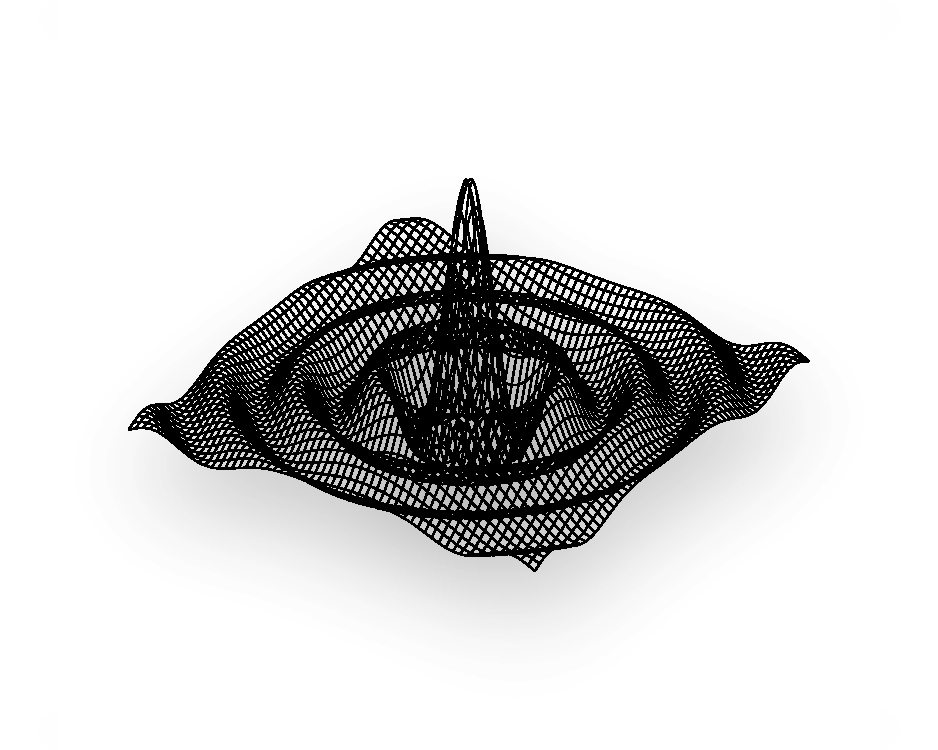
\includegraphics[width=0.88\linewidth,height=0.48\textheight,keepaspectratio]{../figs/pdf/en/fig-03-04.pdf}

% DOCX paragraph 244
\caption{\emph{Una superficie curvada genérica puede ser compleja y tener un radio local de curvatura que
depende de la posición, con un valor positivo o negativo dependiendo de que la superficie sea
convexa o cóncava.}}\label{fig:03-04}
\end{figure}



% DOCX paragraph 246
La teoría de la relatividad general utiliza herramientas matemáticas sofisticadas, muchas de
ellas desarrolladas por matemáticos tales como Tullio Levi-Civita y Gregorio Ricci-Curbastro a
principios del siglo XX, para medir el radio de curvatura y su signo. Gracias a ellos no sería
difícil, por ejemplo, desarrollar apps para nuestros móviles que nos permitieran medir la
curvatura local del espaciotiempo, igual que esas apps que miden el valor local de nuestra
altitud.\index{relatividad general}\index{Levi-Civita, Tullio}\index{Ricci-Curbastro, Gregorio}\index{espaciotiempo!plano}\index{espaciotiempo!curvado}

% DOCX paragraph 247
Los ejemplos vistos hasta ahora nos llevan a una consideración final: hemos visto que es
posible medir el nivel de curvatura de una superficie en dos dimensiones. Lo mismo se puede
hacer para una superficie de tres dimensiones (es decir en un volumen) y, por extensión, en
cuatro dimensiones (como en el espaciotiempo) o incluso en una superficie de dimensiones
arbitrarias. Dicho de otra manera, es posible usar la misma lógica y las mismas herramientas
matemáticas presentadas aquí en dos dimensiones para medir la curvatura del espaciotiempo y
deducir si es plano o no.\index{curvatura|see{espaciotiempo}}

% DOCX paragraph 250
\section{La curvatura y las ecuaciones de Einstein}\label{sec:03-equations}

% DOCX paragraph 252
Ahora que hemos visto lo que es la curvatura y qué herramientas matemáticas se pueden emplear
para medirla, podemos dar un gran paso adelante y descubrir la forma en que la teoría de la
relatividad general vincula estrechamente la presencia de curvatura con la de materia o
energía. Esta vinculación se expresa en las ecuaciones de Einstein propuestas en 1915 y marcó
uno de los capítulos más importantes de la física moderna. Sin embargo, antes de comentar estas
ecuaciones es necesario recordar otra ecuación importante (¡atención al singular!), la cual
también está relacionada con Einstein pero no tiene nada que ver con la gravedad. De hecho, se
introdujo diez años antes de que se propusiera la teoría de la relatividad general, y forma
parte de lo que se llama la teoría de la «relatividad especial» (1905). Esta célebre ecuación
dice:\index{energia@energía}\index{relatividad especial}\index{relatividad!especial|see{relatividad especial}}

% DOCX paragraph 254
\begin{equation}\label{eq:03-02}
E = m\textcolor{gray}{c^{2}}
\end{equation}

% DOCX paragraph 256
Esta expresión, también conocida como la ecuación de Einstein, se ha convertido en un icono de
la contribución científica del físico alemán. Aunque la obtuvo sin tener en mente la gravedad,
expresa una idea importante que usaremos a menudo en el resto del libro. Esencialmente, con el
signo de igualdad, la ecuación \eqref{eq:03-02} afirma la equivalencia entre la energía (E, a
la izquierda del signo igual) y la masa (m, a la derecha). La presencia del cuadrado de la
velocidad de la luz, \emph{c}\textsuperscript{2}, es esencialmente irrelevante para lo que
estamos debatiendo aquí y solo sirve para que los dos lados de la ecuación sean comparables en
términos de unidades (por esta razón se muestra en
gris).\textsuperscript{\hyperlink{note:03-02}{2}} En otras palabras, la ecuación
\eqref{eq:03-02} nos dice que siempre que tenemos una masa (representada por una pluma o por
una roca, por una partícula elemental o una estrella), también tenemos disponible una cierta
cantidad de energía.\index{Einstein!ecuacion@ecuación}\index{energia@energía!equivalencia con la masa}\index{energia@energía}\index{masa!equivalencia con la energia@equivalencia con la energía}

% DOCX paragraph 257
Esta profunda verdad es la clave del funcionamiento de las estrellas, las cuales producen
energía mediante la fusión (en un proceso de fusión termonuclear) de cuatro átomos de hidrógeno
para formar uno de helio, cuya masa es ligeramente inferior a la suma de las masas de los
cuatro átomos de hidrógeno iniciales. Esa pequeña diferencia de masa se libera en forma de
energía. El mismo principio se aplica a las centrales nucleares donde, mediante un proceso de
fisión nuclear, un átomo complejo como el uranio se «rompe» para crear muchos átomos más
pequeños, cuya masa combinada es inferior a la original. De nuevo, la diferencia de masa se
libera en forma de energía.\index{fusion termonuclear@fusión termonuclear}

% DOCX paragraph 258
Esta es la razón por la cual a partir de ahora hablaremos siempre de masa-energía, sin
especificar si se trata de una masa, refiriéndome a un conjunto de partículas elementales
(tales como los electrones, protones o neutrones) a las que podemos asociar una masa en reposo,
o de energía pura.\index{energia@energía!equivalencia con la masa}\index{masa!equivalencia con la energia@equivalencia con la energía}

% DOCX paragraph 259
Ahora sin más preámbulos pasamos a escribir las ecuaciones de Einstein (¡nótese el plural en
este caso!):\index{Einstein!ecuaciones}

% DOCX paragraph 264
\begin{equation}\label{eq:03-03}
G_{\mu\upsilon} = \textcolor{gray}{\left( \frac{8\pi G}{c^{4}} \right)}T_{\mu\upsilon\ \ }
\end{equation}

% DOCX paragraph 266
Es fácil comprender que para la gran mayoría de los lectores, estas ecuaciones están tan claras
como un texto chino; bueno, si no saben leer chino. Es perfectamente normal que a uno le
parezcan incomprensibles estas ecuaciones; habría que hacer un curso universitario completo de
relatividad general para entenderlas. Por ejemplo para el curso que doy en Alemania en
Fráncfort del Meno, necesito la mayor parte de seis meses de clases y la introducción de una
serie de herramientas matemáticas para poder explicar y manipular estas ecuaciones con algo de
detalle.\textsuperscript{\hyperlink{note:03-03}{3}} No obstante, en este caso, podemos evitar
que las matemáticas nos «distraigan» y en lugar de eso concentrarnos en el significado
conceptual más profundo de esas ecuaciones que representan la piedra angular de la teoría
general de la relatividad y por tanto están en el centro de la revolucionaria visión de la
gravedad que tenía Einstein.\index{relatividad general}

% DOCX paragraph 267
Comencemos una vez más con el signo de igualdad en estas ecuaciones \eqref{eq:03-03}. Expresa
la equivalencia entre lo que está del lado izquierdo (el tensor de Einstein,
\emph{G\textsubscript{µν}}) y lo que figura a la derecha. Esto último está formado por dos
partes: una entre paréntesis, que no tiene significado físico y por esta razón se muestra en
gris, y otro tensor, el tensor de energía-momento (\emph{T\textsubscript{µν}}). En esencia, las
ecuaciones de Einstein \eqref{eq:03-03} también se pueden leer como la siguiente ecuación
conceptual:\index{tensor!Einstein}\index{tensor!energia-momento@energía-momento}

% DOCX paragraph 270
\begin{equation}\label{eq:03-04}
(\text{tensor de Einstein}) = (\text{tensor de energía-momento})
\end{equation}

% DOCX paragraph 271
% Equation number is generated with the preceding equation.

% DOCX paragraph 273
Como el tensor de Einstein representa una medida de la curvatura del espaciotiempo (de hecho,
es proporcional al tensor de Riemann), mientras que el tensor de energía-momento proporciona
una medida de la cantidad de materia-energía presente en el espaciotiempo (cuanto mayor sea la
materia y su concentración, mayor será este tensor), las complejas ecuaciones \eqref{eq:03-03}
esencialmente afirman que:

% DOCX paragraph 276
\begin{equation}\label{eq:03-05}
(\text{geometría-curvatura}) = (\text{masa-energía})
\end{equation}

% DOCX paragraph 277
% Equation number is generated with the preceding equation.

% DOCX paragraph 279
Se puede decir que este es el concepto más importante de todo el libro. Expresa exactamente lo
que contienen las ecuaciones de Einstein \eqref{eq:03-03} de una manera más compleja pero
también más elegante en cuanto a las matemáticas y revolucionaria para la física. Dicho de otro
modo, en cualquier lugar en el que haya materia (o energía), encontraremos una curvatura del
espaciotiempo. Esto es verdad siempre, tanto si hablamos de la masa de una galaxia como de un
grano de arena, de un rayo de luz o de una bola de cañón. Solo variará la magnitud de esta
curvatura, es decir, el que sea más o menos pronunciada. En el siguiente capítulo, aprenderemos
cómo distinguir curvaturas de diferentes intensidades y comprenderemos cómo la naturaleza es
capaz de producirlas. Pero primero tenemos que ver cómo encaja la gravedad en el marco
conceptual que acabamos de comentar.\index{energia@energía!equivalencia con la masa}\index{masa!equivalencia con la energia@equivalencia con la energía}

% DOCX paragraph 282
\section{El espaciotiempo es una tela elástica}\label{sec:03-fabric}

% DOCX paragraph 284
Aun siendo rica en importantes implicaciones que exploraremos en el resto del libro, la
ecuación \eqref{eq:03-05} sigue sin explicar cómo casa la gravedad con lo que se ha dicho hasta
ahora. En otras palabras, probablemente aún no esté claro cómo las ecuaciones de Einstein,
resumidas por la ecuación \eqref{eq:03-05}, pueden explicar las causas por las que una manzana
cae del árbol. Este es el siguiente paso conceptual que tenemos que dar y que requerirá un poco
más de concentración.

% DOCX paragraph 285
Para comprender de qué manera están ligadas inextricablemente la curvatura y la gravedad,
empecemos por imaginar una superficie plana pero elástica y deformable, por ejemplo la sábana
de una cama recién hecha. En ausencia de pesos, se la ve perfectamente lisa y plana, y así
permanece hasta que algo perturbe su superficie. Esto se muestra en la figura~\ref{fig:03-05},
la cual también nos ayuda a entender el significado de las ecuaciones de Einstein: la ausencia
de materia-energía conduce a un espaciotiempo con curvatura cero y por tanto plano. Dentro de
dicho espaciotiempo podemos tomar un vector, transportarlo paralelamente a lo largo de un
circuito cerrado y, al final del proceso nos encontramos con que es idéntico al vector inicial.\index{vector}

% DOCX paragraph 286
\begin{figure}[htbp]
\centering
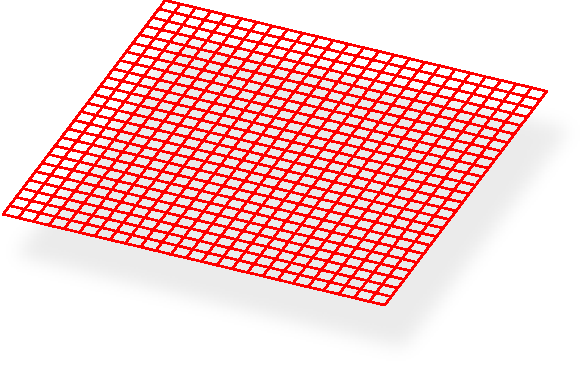
\includegraphics[width=0.88\linewidth,height=0.48\textheight,keepaspectratio]{../figs/pdf/en/fig-03-05.pdf}

% DOCX paragraph 287
\caption{\emph{La ausencia de materia-energía produce un espaciotiempo sin curvatura que por tanto es plano.}}\label{fig:03-05}
\end{figure}



% DOCX paragraph 288
Si nos ponemos puntillosos, un espaciotiempo de este tipo (estrictamente vacío) no puede
existir ya que la presencia de materia o energía, incluso si es infinitesimal, crearía una
perturbación y eliminaría la «planitud» absoluta. No obstante, el ejemplo es útil porque a
menudo es posible considerar un espaciotiempo «casi plano» o «localmente plano» que, aun no
siendo plano a gran escala, es plano en una pequeña región.\index{espaciotiempo!plano}

% DOCX paragraph 289
Intentemos ahora imaginar qué sucedería si colocáramos un objeto pesado en esta sábana por
ejemplo una bola de bolos. Como es fácil de adivinar, se «curvaría» alrededor del peso,
exactamente como se aprecia en la figura~\ref{fig:03-06}. Este ejemplo nos ofrece una analogía
útil con lo que expresan las ecuaciones de Einstein: la presencia de materia (o energía)
produce un espaciotiempo con curvatura no nula, y por tanto está curvado. Si tomáramos un
vector y lo transportáramos en paralelo a lo largo de un circuito cerrado dentro de él, al
final del recorrido nos encontraríamos con que es diferente del
inicial.\textsuperscript{\hyperlink{note:03-04}{4}}\index{energia@energía!equivalencia con la masa}\index{masa!equivalencia con la energia@equivalencia con la energía}\index{espaciotiempo!curvado}

% DOCX paragraph 291
\begin{figure}[htbp]
\centering
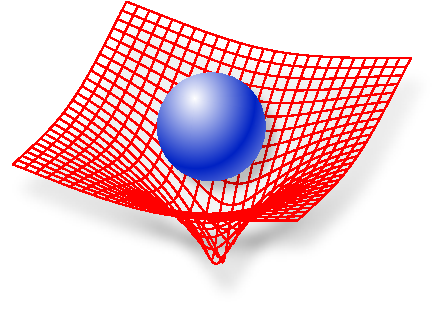
\includegraphics[width=0.88\linewidth,height=0.48\textheight,keepaspectratio]{../figs/pdf/en/fig-03-06.pdf}
\caption{\emph{La presencia de materia-energía (representada aquí por una esfera que podría ser un planeta o
un grano de arena) produce un espaciotiempo con curvatura no nula, o sea, curvado.}}\label{fig:03-06}
\end{figure}



% DOCX paragraph 292
El ejemplo de la sábana nos brinda la oportunidad de hacer tres observaciones. La primera tiene
que ver con un aspecto esencial de la figura~\ref{fig:03-06} que no debemos pasar por alto: la
curvatura producida por la bola de bolos no es idéntica en todas partes sino que varía de un
punto a otro. En particular, es muy pequeña en los bordes de la sábana, que parecerá
prácticamente plana, y más pronunciada si se acerca al punto donde está situado el objeto, y
donde alcanzará su tamaño máximo. En otras palabras, es natural esperar que, en condiciones
genéricas, la curvatura es una función de la posición: solo en circunstancias excepcionales
(como en el caso de la esfera bidimensional) es constante la curvatura.\index{esfera bidimensional}

% DOCX paragraph 293
La segunda consideración está relacionada con la «forma» de la deformación. Aunque pueda
parecer obvio que la presencia de una bola de bolos da lugar a una curvatura cóncava o
positiva, las ecuaciones de Einstein revelan que también es posible tener, de manera totalmente
equivalente, una curvatura convexa o negativa. Nuestra experiencia es que la materia que nos
rodea y con la que normalmente realizamos los experimentos de hecho produce una curvatura
positiva exactamente tal como ilustra la figura~\ref{fig:03-06}. Ahora bien, y esto es algo que
permiten las ecuaciones de Einstein: no puede excluirse la existencia de materia que produzca
una curvatura negativa.

% DOCX paragraph 294
La observación tercera y final se refiere al impacto de la curvatura. Es importante darse
cuenta de que la presencia de una curvatura afectará a la dinámica (es decir, el movimiento) de
cualquier objeto en sus alrededores. Por ejemplo, imaginemos que añadimos otra esfera más
pequeña y más ligera al lado de la bola de bolos, de tal forma que no produzca una curvatura en
la sábana comparable a la primera. En este escenario, y en ausencia de fricción, el segundo
objeto se verá obligado a trasladarse, cayendo hacia el centro de la curvatura producida por la
bola de bolos. Con este ejemplo podemos pues comprender cómo la gravedad se manifiesta en
términos geométricos. Al modificar el espaciotiempo en el cual ocurre el movimiento, la
curvatura produce una variación en la dinámica de los cuerpos, que de otra manera permanecerían
en el estado de movimiento rectilíneo o en reposo.

% DOCX paragraph 297
\section{Curvatura y gravedad}\label{sec:03-gravity}

% DOCX paragraph 299
Habiendo presentado y debatido los conceptos de espaciotiempo y de curvatura, finalmente
estamos listos para regresar a aquella afirmación sencilla pero oscura \eqref{eq:03-01}.
Recuerdo que decía:

% DOCX paragraph 300
\[
\begin{pmatrix}\text{la gravedad es la manifestación} \\ \text{de la curvatura del espaciotiempo}\end{pmatrix}
\]

% DOCX paragraph 302
Llegados a este punto en mi curso de relatividad general, las miradas de desconcierto y
escepticismo que aparecen en los rostros de mis estudiantes cuando se encuentran por primera
vez con esta afirmación se tornan sutiles sonrisas de satisfacción. La expresión de alguien que
se da cuenta de que «¡Claro! ¿Cómo podía ser de otra manera?» La frase no solo ha dejado de ser
críptica, sino que se ha vuelto profundamente fascinante.

% DOCX paragraph 303
Dicho de otro modo, Einstein ha afirmado que si el espaciotiempo está vacío en el sentido de
estar desprovisto de cualquier materia que produce curvatura, entonces también es plano. En
este caso todos los objetos en dicho espaciotiempo mantendrán su estado de movimiento: según
sus condiciones iniciales, seguirán estacionarios o se trasladarán a velocidad constante a lo
largo de una línea recta (efectivamente, es el principio de inercia). Ahora bien, si el
espaciotiempo contiene materia-energía que produzca una curvatura, entonces todos los objetos
en el espaciotiempo se verán afectados por esta curvatura a través de una modificación de su
estado de movimiento. Así pues, los objetos que inicialmente estaban en reposo ya no podrán
permanecer así. Por otra parte, aquellos objetos que se mueven a velocidad constante a lo largo
de una línea recta modificarán su trayectoria y velocidad.\index{energia@energía!equivalencia con la masa}\index{masa!equivalencia con la energia@equivalencia con la energía}

% DOCX paragraph 304
Se sigue que, desde esta perspectiva diferente y decididamente revolucionaria de la gravedad,
si la manzana cae del árbol no es porque una fuerza gravitatoria la atraiga hacia la Tierra. Lo
que ocurre es que la Tierra, con su contenido de materia y energía, curva el espaciotiempo
alrededor de sí misma y obliga a los objetos a moverse de manera correspondiente. Cuando la
manzana ya no está sujeta al árbol, el cual hasta entonces impedía que se moviera libremente,
solo puede moverse siguiendo la curvatura local del espaciotiempo y por tanto hacia el centro
de la Tierra. ¡Y eso es efectivamente lo que hace! Bueno, al menos hasta que se encuentra con
la superficie del planeta, el cual le impide continuar. Eso es lo que la figura~\ref{fig:03-07}
muestra de una manera esquemática (y por supuesto sin respetar la escala).\index{manzana (caida)@manzana (caída)}\index{fuerza!gravitatoria}

% DOCX paragraph 306
\begin{figure}[htbp]
\centering
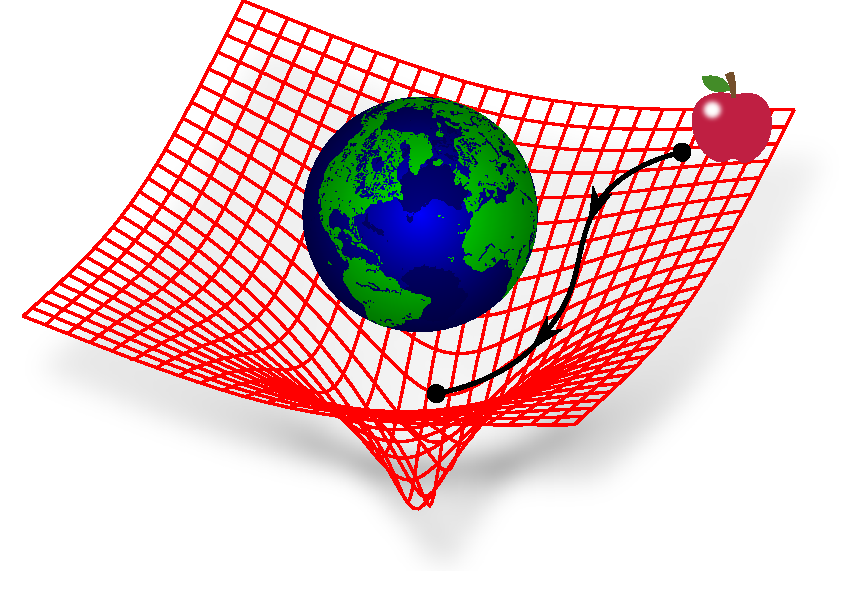
\includegraphics[width=0.88\linewidth,height=0.48\textheight,keepaspectratio]{../figs/pdf/en/fig-03-07.pdf}
\caption{\emph{Interpretación de la caída de una manzana en la teoría de la gravitación de Einstein: la Tierra
produce una curvatura en el espaciotiempo, y la manzana tiene que moverse siguiéndola,
«cayendo» hacia el centro del planeta.}}\label{fig:03-07}
\end{figure}



% DOCX paragraph 307
Aquí se podría añadir un comentario adicional, que la lectora o el lector entenderá
perfectamente a estas alturas. La razón, una vez liberada del árbol, por la cual la manzana no
se mueve hacia el espacio interplanetario va ligada al signo de la curvatura, es decir, al
hecho de que la Tierra produzca una curvatura positiva (o cóncava). Sin embargo, si admitimos
hipotéticamente la existencia de un tipo de materia que produzca una curvatura negativa
entonces la superficie de la «sábana» de la figura~\ref{fig:03-06} se deformaría con una
curvatura convexa, y la gravedad se comportaría de la manera opuesta: no sería atractiva sino
repulsiva y ¡la manzana volaría al espacio! Afortunadamente, incluso en presencia de este
«cambio de signo», el título de este libro seguiría siendo válido. De hecho, en este caso ¡la
gravedad aún sería más atractiva para nuestra atención!

% DOCX paragraph 308
El ejemplo recién sugerido de una gravedad repulsiva puede parecer absurdo a primera vista,
pero esto es exactamente lo que pensamos que está ocurriendo ahora mismo en el universo como un
todo. Observando explosiones de supernova muy distantes, es posible deducir que el universo se
encuentra actualmente en una fase de expansión acelerada. La causa de este fenómeno todavía no
está clara, pero podría estar vinculada a la energía oscura: una forma de energía tenue que
generaría una curvatura negativa. El resultado es que, al menos a escala cósmica, en apariencia
produciría una acción ¡similar a la antigravedad!\index{supernova}\index{energia@energía!oscura}\index{energia oscura@energía oscura}\index{antigravedad}

% DOCX paragraph 311
\section{Nada se mueve en línea recta}\label{sec:03-geodesics}

% DOCX paragraph 313
Ya hemos comentado en la nota 4 el error lógico que contiene el ejemplo de la
figura~\ref{fig:03-06}. Allí, para explicar la curvatura y la gravedad, utilizamos una bola de
bolos ya inmersa en un campo gravitatorio (el terrestre) de tal manera que curva la sábana
precisamente porque ya está en un campo así. Por tanto, estamos usando la dinámica de un objeto
en un campo gravitatorio para explicar qué es la curvatura, que podemos decir que es el
auténtico origen de la gravedad. La circularidad del argumento es evidente. Afortunadamente,
sin embargo, esta circularidad también es inofensiva: tan solo nos muestra que la analogía de
la sábana curvada es valiosa pero no perfecta.

% DOCX paragraph 314
De hecho puede utilizarse una analogía mejor para visualizar y medir la curvatura sin ayuda de
sábanas ni bolas de bolos. Pero aún necesito un poco de atención de los lectores para hacer
esto: les aseguro que merecerá la pena, pues descubriremos una de las herramientas más útiles
de la astronomía moderna.

% DOCX paragraph 315
Volvamos a la idea de un espaciotiempo vacío y por tanto plano donde un objeto sigue el
principio de inercia: permanece estacionario si inicialmente estaba estacionario o continúa con
su movimiento rectilíneo uniforme (es decir, a velocidad constante). Sin embargo, está claro
que esto ya no puede ser verdad si el espaciotiempo está curvado. En este caso, la curvatura
modificará la trayectoria del objeto, y esta tendrá que adaptarse consecuentemente. Así pues,
el movimiento rectilíneo uniforme ya no puede existir en un espaciotiempo curvado, donde cada
movimiento será necesariamente curvado. En otras palabras, nada se mueve en línea recta en un
espaciotiempo que contenga materia-energía excepto tratándose de distancias infinitesimales.

% DOCX paragraph 316
La conclusión que acabamos de alcanzar tiene dos consecuencias interesantes. La primera se
relaciona con la experiencia común de que una línea recta representa la distancia mínima entre
dos puntos, la denominada geodésica. Obviamente esto se cumple en un espaciotiempo plano pero
deja de ser verdadero en un espaciotiempo curvado en el cual una línea recta ya no representa
la distancia mínima.\index{geodesica@geodésica}

% DOCX paragraph 317
Esta consideración es menos extraña de lo que puede parecer, y dos ejemplos concretos nos
ayudarán a darnos cuenta de que es bastante obvio. Lo primero, supongamos que el viajero se
mueve a lo largo de una superficie curvada y debe ir del punto A al punto B, como se muestra en
la figura~\ref{fig:03-08}.

% DOCX paragraph 318
\begin{figure}[htbp]
\centering
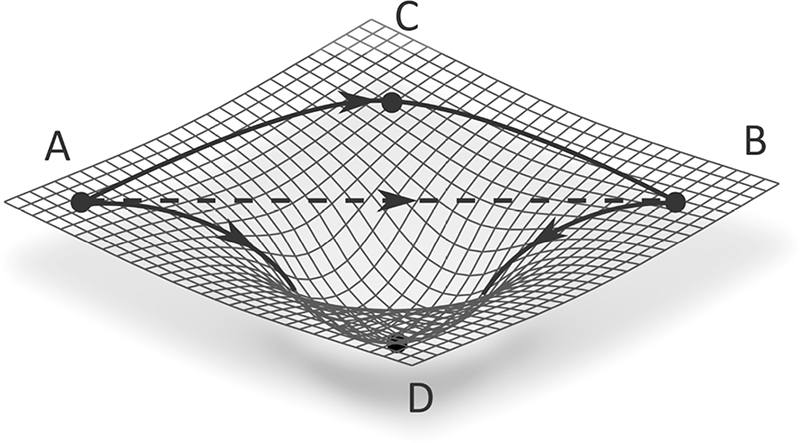
\includegraphics[width=0.88\linewidth,height=0.48\textheight,keepaspectratio]{../figs/source/en/fig-03-08.png}

% DOCX paragraph 320
\caption{\emph{En un espaciotiempo curvado, una línea recta no es el camino más corto para unir dos puntos (es
decir, una geodésica). En la figura, el recorrido ACB es la geodésica entre A y B.\index{geodesica@geodésica}}}\label{fig:03-08}
\end{figure}



% DOCX paragraph 322
La situación es similar a la de caminar por las colinas cerca de Trieste, en Italia, donde son
muy comunes este tipo de deformaciones del terreno. Obviamente no se puede alcanzar el punto B
desde A en una línea recta (a menos que sea volando, pero eso lo consideraremos en el próximo
ejemplo); habría que seguir la superficie del terreno por la ruta ACB o ADB, eligiendo la más
corta y menos fatigosa. Para aclararlo, supongamos que es la primera, aunque en otras
condiciones podría ser la segunda. En este caso, la ruta ACB representa la geodésica entre A y
B, la curva que, al recorrerla, mide la distancia más corta entre los dos puntos A y
B.\textsuperscript{\hyperlink{note:03-05}{5}}\index{geodesica@geodésica}

% DOCX paragraph 323
Para el segundo ejemplo, basta pensar en las rutas que siguen los aviones o los barcos para
desplazarse de un punto a otro de nuestro planeta. Estas rutas también representan geodésicas,
ya que se calculan para minimizar el gasto de combustible y, por tanto, trazan la distancia más
corta entre los dos puntos. Sin embargo, puesto que los aviones y los barcos siguen estando
obligados a moverse por la superficie curva de la Tierra, estas geodésicas no pueden ser líneas
rectas: han de ser curvas, es decir, las geodésicas de un espaciotiempo curvado. Esto tiene una
consecuencia importante: hemos visto que es posible aproximar localmente un espaciotiempo
curvado por uno plano; por el mismo principio, parecerá que los aviones y los barcos se mueven
por trayectorias rectas a escalas de longitud pequeñas, aunque en realidad son curvas a escalas
comparables al radio de curvatura de la Tierra.

% DOCX paragraph 324
La segunda consecuencia importante de la conclusión de que nada se mueve en línea recta está
vinculada con la astronomía. Las observaciones nos dicen que el universo está fundamentalmente
vacío, con la excepción de unas concentraciones locales de materia, las cuales se manifiestan
en forma de planetas, estrellas, galaxias, cúmulos de galaxias etc. Así pues, en el
espaciotiempo que describe nuestro universo, hay vastas regiones (que representan la mayor
parte del volumen espacial) que son casi planas. En estas regiones, los objetos con masa se
desplazan a lo largo de las líneas rectas que siguen siendo paralelas si lo estaban
inicialmente. Pero en aquellas regiones donde la materia está presente, que son mucho menos
frecuentes y representan una pequeña fracción del volumen espacial, el espaciotiempo, por el
contrario, está curvado y la trayectoria de los objetos con masa no puede ser rectilínea: dos
senderos que comienzan paralelos necesariamente divergirán o convergerán.\index{espaciotiempo!plano (casi)}

% DOCX paragraph 325
Basándonos en estas consideraciones, podemos «fácilmente» crear herramientas que nos permitan
verificar si el espaciotiempo es realmente plano o curvado, incluso sin recurrir a la ayuda de
sábanas y bolas de bolos. Sería «suficiente» tomar pequeños objetos con masa, por ejemplo
microsatélites, y lanzarlos hacia un cuerpo celeste bastante distante, como Próxima Centauri
(la estrella más cercana a nosotros después del Sol, que está a 4,24 años luz) asegurándose de
que las trayectorias sean inicialmente paralelas. En este punto, sería suficiente con comprobar
la separación entre los objetos cuando han alcanzado su destino, en nuestro caso después de
unos 270 000 años (suponiendo que se mueven a la máxima velocidad que ha alcanzado hasta ahora
un satélite artificial). Dependiendo de si la separación ha disminuido o aumentado en
comparación con la inicial, sabremos si estos se han encontrado durante el viaje con regiones
del espaciotiempo con curvatura positiva o negativa.\index{Proxima Centauri@Próxima Centauri}

% DOCX paragraph 326
Este ejemplo es muy poco realista. Aunque conceptualmente correcto, es imposible en la
práctica; es solo una idea abstrusa de un físico teórico. Sin embargo hace cien años Einstein
sugirió un experimento conceptualmente similar y también factible con la tecnología de la
época. De hecho con ese experimento convenció incluso a los científicos más escépticos de
aquella época de que su extraña teoría de la gravitación era correcta.

% DOCX paragraph 327
Para comprender mejor lo que proponía Einstein, tenemos que volver a su ecuación sobre la
equivalencia entre masa y energía, es decir la ecuación \eqref{eq:03-02}. Aquella ecuación nos
permite deducir que, si en un espaciotiempo curvado, el movimiento de un objeto con masa no es
rectilíneo, lo mismo valdrá para el movimiento de un objeto sin masa, por ejemplo un rayo de
luz, al que también llamamos fotón. En otras palabras, un rayo de luz que se propaga en un
espaciotiempo curvo tendrá necesariamente que seguir una trayectoria curvada. Con el riesgo de
ser pedante, pero con la intención de ser extraordinariamente preciso, debería subrayar que un
rayo de luz siempre se mueve a lo largo de una geodésica, una línea de separación mínima. Esta
línea será una línea recta solamente en un espaciotiempo plano, y una línea curvada en
condiciones más generales, como las que se dan en un espaciotiempo curvado.\index{foton@fotón}\index{geodesica@geodésica}

% DOCX paragraph 328
En comparación con los satélites, los fotones ofrecen dos ventajas adicionales: son mucho más
rápidos que cualquier objeto con masa (de hecho viajan a la máxima velocidad permitida); y los
emiten en abundancia los cuerpos celestes como Próxima Centauri. Por tanto todo lo que hay que
hacer es usar telescopios para interceptar estos fotones y deducir si su trayectoria se ha
modificado o no en la presencia de una curvatura.\index{Proxima Centauri@Próxima Centauri}

% DOCX paragraph 329
Esto es exactamente lo que propuso Einstein hace unos cien años con ocasión del famoso eclipse
solar total de 1919, un experimento cuya idea básica se muestra en la figura~\ref{fig:03-09}.
Esencialmente, hizo una consideración de gran inteligencia: si un rayo de luz es desviado por
la presencia de un objeto masivo (por ejemplo, el Sol) que curva el espaciotiempo y tiene
tendencia a «atraer» el rayo, en principio ¡es posible «ver» lo que hay detrás del objeto!\index{Sol!eclipse (vease eclipse solar)@eclipse (véase eclipse solar)}\index{eclipse solar}

% DOCX paragraph 330
Obviamente, la habilidad de desviar un rayo de luz depende de la intensidad de la curvatura que
produce el cuerpo celeste y por ello (como se verá en el próximo capítulo) depende también de
su masa y radio. Trabajando un poco con una versión aproximada de sus ecuaciones, Einstein
concluyó que si bien no era posible observar objetos situados exactamente detrás del Sol, la
curvatura generada por nuestra estrella sería suficiente para que nos mostrara objetos cercanos
a su superficie proyectada.

% DOCX paragraph 331
En este punto, solo quedaba un problema por resolver: el Sol es la fuente dominante de luz
alrededor de nosotros y por tanto es imposible identificar la pequeña aportación a la
luminosidad de una estrella cerca del borde. Para comprobar esta idea, ¡tendríamos que apagar
el Sol! Afortunadamente para nosotros, eso no se puede hacer, pero es esencialmente lo que
sucede durante un eclipse total. En ese caso, la luz que nos llega del Sol está prácticamente
suprimida, de manera que se pueden ver los objetos celestes próximos a la superficie
proyectada; bueno, ¡al menos según la relatividad general! Por tanto, el experimento sugerido
por Einstein consistía en observar un eclipse solar total desde una posición óptima y
determinar cuáles de las estrellas próximas al borde y teóricamente invisibles al estar
cubiertas por el Sol eran sin embargo visibles.\index{relatividad general}\index{eclipse solar}

% DOCX paragraph 334
\begin{figure}[htbp]
\centering
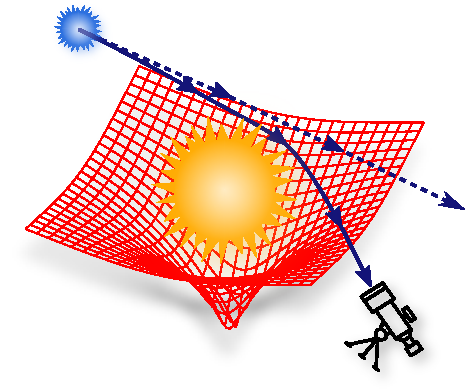
\includegraphics[width=0.88\linewidth,height=0.48\textheight,keepaspectratio]{../figs/pdf/en/fig-03-09.pdf}

% DOCX paragraph 335
\caption{\emph{Una de las predicciones más importantes de Einstein es que la luz no puede viajar en línea
recta en un espaciotiempo curvado. Por ello es posible observar cuerpos celestes incluso cuando
los ocultan otros objetos situados en primer plano.}}\label{fig:03-09}
\end{figure}



% DOCX paragraph 336
Omito los detalles históricos de una expedición aventurera liderada por el astrónomo inglés Sir
Arthur Eddington, gran admirador de Einstein y uno de los pocos que desde el principio apoyaron
la teoría de la relatividad general. Las observaciones que hizo Eddington el 29 de mayo de 1919
en la isla de Príncipe, por aquel entonces territorio portugués y actualmente parte de la
República Democrática de Santo Tomé y Príncipe (un archipiélago del Atlántico situado en el
golfo de Guinea) revelaron que era efectivamente posible medir una desviación de luz producida
por estrellas distantes y que esta era igual a unos 1,75 arcosegundos. La medida de un fenómeno
físico imposible según la gravedad de Newton, pero que coincidía con lo que había predicho la
revolucionaria teoría de la relatividad general fue la gota que colmó el vaso para la teoría de
Newton y supuso la consagración científica de todas las ideas «extrañas» que hemos comentado en
este capítulo: espaciotiempo, energía, materia, curvatura … Claramente, ¡esas ideas no eran
extrañas en absoluto!\index{Eddington, sir Arthur}\index{Eddington, sir Arthur}\index{relatividad general}

% DOCX paragraph 337
El fenómeno que acabo de describir (que la luz no puede propagarse en línea recta en un
espaciotiempo curvado) es una de las aplicaciones más útiles de la teoría del brillante físico
alemán, hasta tal punto que se ha hecho un chiste llamándola «el regalo de Einstein a la
astronomía». Es fácil entender la razón de esta afirmación. Igual que el Sol, de hecho,
cualquier objeto astronómico puede actuar como una lente gravitatoria, desviando la luz que
viene de otros objetos y no solo distorsionando su apariencia sino también amplificándola,
haciendo así visibles aquellos objetos cuya imagen de otra manera sería demasiado débil. Esto
es exactamente lo que hace una lente: concentra un haz de rayos de luz paralelos en un punto:
su foco.

% DOCX paragraph 338
Aprovechando estos interesantes efectos de desviación, los astrónomos pueden obtener ahora
múltiples imágenes amplificadas de galaxias a inmensas distancias de nosotros, trabajando con
lo que se suele llamar efecto de lente gravitatoria.\index{lentes gravitatorias!efecto}\index{efecto de lente|see{lentes gravitatorias}}

% DOCX paragraph 339
Un comentario final: quiero señalar que este fenómeno también puede darse cuando el objeto que
actúa como lente no es visible porque no emite luz, aun siendo bastante masivo. En este caso,
la presencia de un «objeto lente» se puede deducir de la curvatura del espaciotiempo que
induce, y que se manifiesta a través de la distorsión de imágenes de otros objetos lejanos. Un
ejemplo clásico de este tipo de efecto de lente gravitatoria es el fenómeno producido por la
llamada materia oscura, que no emite luz. En cambio, su presencia es detectable por medio de la
acción gravitatoria que produce a escala galáctica al afectar a la velocidad a la cual giran
las estrellas en galaxias en espiral alrededor del centro, y revelando su presencia en forma de
un enorme halo esférico.\index{materia oscura}

% DOCX paragraph 358
\begin{figure}[htbp]
\centering
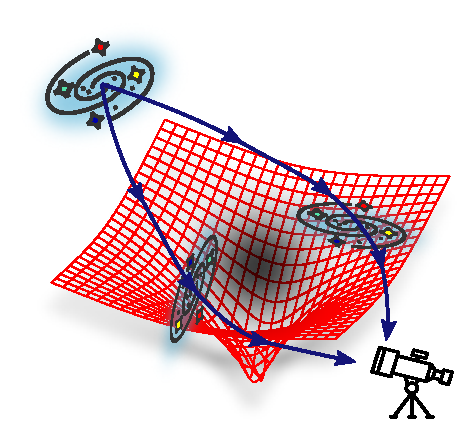
\includegraphics[width=0.88\linewidth,height=0.48\textheight,keepaspectratio]{../figs/pdf/en/fig-03-10.pdf}
\caption{\emph{Los objetos astronómicos compactos pueden actuar como lentes gravitatorias y concentrar
emisiones desde fuentes lejanas o producir imágenes múltiples. Las lentes gravitatorias también
pueden ser invisibles, como en el caso de la materia oscura.\index{materia oscura}}}\label{fig:03-10}
\end{figure}



% DOCX paragraph 360
La figura~\ref{fig:03-10} ilustra de forma esquemática cómo la presencia de materia oscura,
aunque invisible, produce una curvatura del espaciotiempo local, la cual genera múltiples
imágenes distorsionadas de galaxias lejanas. En este caso, analizando cómo se distorsionan las
imágenes de los objetos celestes, las observaciones pueden ser útiles para estudiar las
propiedades de la materia oscura, tales como su masa y distribución.\index{materia oscura}

% DOCX paragraph 361
Pero el asunto no acaba aquí. En el capítulo 7 veremos cómo la desviación de un haz de luz en
las proximidades de un espaciotiempo muy curvado da lugar a fenómenos curiosos tales como
imágenes dobles y triples, amplificaciones y absorciones. En el mismo capítulo también
explicaré cómo es posible obtener la imagen de un agujero negro, como lo ha hecho
recientemente mi grupo de investigación en colaboración con el Telescopio del Horizonte de
Sucesos (Event Horizon Telescope).
